%----------------------------------------------------------------------------------------
%	PACKAGES AND OTHER DOCUMENT CONFIGURATIONS
%----------------------------------------------------------------------------------------

\documentclass[11pt,fleqn]{book} % Default font size and left-justified equations

\usepackage[top=3cm,bottom=3cm,left=3.2cm,right=3.2cm,headsep=10pt,letterpaper]{geometry} % Page margins

\usepackage{xcolor} % Required for specifying colors by name
\definecolor{ocre}{RGB}{52,177,201} % Define the orange color used for highlighting throughout the book%

% Font Settings
\usepackage{avant} % Use the Avantgarde font for headings
%\usepackage{times} % Use the Times font for headings
\usepackage{mathptmx} % Use the Adobe Times Roman as the default text font together with math symbols from the Sym­bol, Chancery and Com­puter Modern fonts
\usepackage{microtype} % Slightly tweak font spacing for aesthetics
\usepackage[utf8]{inputenc} % Required for including letters with accents
\usepackage[T1]{fontenc} % Use 8-bit encoding that has 256 glyphs
\usepackage{amsthm}
%%%

% Bibliography
\usepackage[style=alphabetic,sorting=nyt,sortcites=true,autopunct=true,babel=hyphen,hyperref=true,abbreviate=false,backref=true,backend=biber]{biblatex}
\addbibresource{bibliography.bib} % BibTeX bibliography file
\defbibheading{bibempty}{}

%----------------------------------------------------------------------------------------
%	VARIOUS REQUIRED PACKAGES
%----------------------------------------------------------------------------------------

\usepackage{titlesec} % Allows customization of titles

\usepackage{graphicx} % Required for including pictures
\graphicspath{{Pictures/}} % Specifies the directory where pictures are stored
% \graphicspath{{Plots/}}
\usepackage{lipsum} % Inserts dummy text

\usepackage{tikz} % Required for drawing custom shapes

\usepackage[english]{babel} % English language/hyphenation

\usepackage{enumitem} % Customize lists
\setlist{nolistsep} % Reduce spacing between bullet points and numbered lists

\usepackage{booktabs} % Required for nicer horizontal rules in tables

\usepackage{eso-pic} % Required for specifying an image background in the title page

%----------------------------------------------------------------------------------------
%	MAIN TABLE OF CONTENTS
%----------------------------------------------------------------------------------------

\usepackage{titletoc} % Required for manipulating the table of contents

\contentsmargin{0cm} % Removes the default margin
% Chapter text styling
\titlecontents{chapter}[1.25cm] % Indentation
{\addvspace{15pt}\large\sffamily\bfseries} % Spacing and font options for chapters
{\color{ocre!60}\contentslabel[\Large\thecontentslabel]{1.25cm}\color{ocre}} % Chapter number
{}  
{\color{ocre!60}\normalsize\sffamily\bfseries\;\titlerule*[.5pc]{.}\;\thecontentspage} % Page number
% Section text styling
\titlecontents{section}[1.25cm] % Indentation
{\addvspace{5pt}\sffamily\bfseries} % Spacing and font options for sections
{\contentslabel[\thecontentslabel]{1.25cm}} % Section number
{}
{\sffamily\hfill\color{black}\thecontentspage} % Page number
[]
% Subsection text styling
\titlecontents{subsection}[1.25cm] % Indentation
{\addvspace{1pt}\sffamily\small} % Spacing and font options for subsections
{\contentslabel[\thecontentslabel]{1.25cm}} % Subsection number
{}
{\sffamily\;\titlerule*[.5pc]{.}\;\thecontentspage} % Page number
[] 

%----------------------------------------------------------------------------------------
%	MINI TABLE OF CONTENTS IN CHAPTER HEADS
%----------------------------------------------------------------------------------------

% Section text styling
\titlecontents{lsection}[0em] % Indendating
{\footnotesize\sffamily} % Font settings
{}
{}
{}

% Subsection text styling
\titlecontents{lsubsection}[.5em] % Indentation
{\normalfont\footnotesize\sffamily} % Font settings
{}
{}
{}
 
%----------------------------------------------------------------------------------------
%	PAGE HEADERS
%----------------------------------------------------------------------------------------

\usepackage{fancyhdr} % Required for header and footer configuration

\pagestyle{fancy}
\renewcommand{\chaptermark}[1]{\markboth{\sffamily\normalsize\bfseries\chaptername\ \thechapter.\ #1}{}} % Chapter text font settings
\renewcommand{\sectionmark}[1]{\markright{\sffamily\normalsize\thesection\hspace{5pt}#1}{}} % Section text font settings
\fancyhf{} \fancyhead[LE,RO]{\sffamily\normalsize\thepage} % Font setting for the page number in the header
\fancyhead[LO]{\rightmark} % Print the nearest section name on the left side of odd pages
\fancyhead[RE]{\leftmark} % Print the current chapter name on the right side of even pages
\renewcommand{\headrulewidth}{0.5pt} % Width of the rule under the header
\addtolength{\headheight}{2.5pt} % Increase the spacing around the header slightly
\renewcommand{\footrulewidth}{0pt} % Removes the rule in the footer
\fancypagestyle{plain}{\fancyhead{}\renewcommand{\headrulewidth}{0pt}} % Style for when a plain pagestyle is specified

% Removes the header from odd empty pages at the end of chapters
\makeatletter
\renewcommand{\cleardoublepage}{
\clearpage\ifodd\c@page\else
\hbox{}
\vspace*{\fill}
\thispagestyle{empty}
\newpage
\fi}

%----------------------------------------------------------------------------------------
%	THEOREM STYLES
%----------------------------------------------------------------------------------------

\usepackage{amsmath,amsfonts,amssymb,amsthm} % For math equations, theorems, symbols, etc

\newcommand{\intoo}[2]{\mathopen{]}#1\,;#2\mathclose{[}}
\newcommand{\ud}{\mathop{\mathrm{{}d}}\mathopen{}}
\newcommand{\intff}[2]{\mathopen{[}#1\,;#2\mathclose{]}}
\newtheorem{notation}{Notation}[chapter]

%%%%%%%%%%%%%%%%%%%%%%%%%%%%%%%%%%%%%%%%%%%%%%%%%%%%%%%%%%%%%%%%%%%%%%%%%%%
%%%%%%%%%%%%%%%%%%%% dedicated to boxed/framed environements %%%%%%%%%%%%%%
%%%%%%%%%%%%%%%%%%%%%%%%%%%%%%%%%%%%%%%%%%%%%%%%%%%%%%%%%%%%%%%%%%%%%%%%%%%
\newtheoremstyle{ocrenumbox}% % Theorem style name
{0pt}% Space above
{0pt}% Space below
{\normalfont}% % Body font
{}% Indent amount
{\small\bf\sffamily\color{ocre}}% % Theorem head font
{\;}% Punctuation after theorem head
{0.25em}% Space after theorem head
{\small\sffamily\color{ocre}\thmname{#1}\nobreakspace\thmnumber{\@ifnotempty{#1}{}\@upn{#2}}% Theorem text (e.g. Theorem 2.1)
\thmnote{\nobreakspace\the\thm@notefont\sffamily\bfseries\color{black}---\nobreakspace#3.}} % Optional theorem note
\renewcommand{\qedsymbol}{$\blacksquare$}% Optional qed square

\newtheoremstyle{blacknumex}% Theorem style name
{5pt}% Space above
{5pt}% Space below
{\normalfont}% Body font
{} % Indent amount
{\small\bf\sffamily}% Theorem head font
{\;}% Punctuation after theorem head
{0.25em}% Space after theorem head
{\small\sffamily{\tiny\ensuremath{\blacksquare}}\nobreakspace\thmname{#1}\nobreakspace\thmnumber{\@ifnotempty{#1}{}\@upn{#2}}% Theorem text (e.g. Theorem 2.1)
\thmnote{\nobreakspace\the\thm@notefont\sffamily\bfseries---\nobreakspace#3.}}% Optional theorem note

\newtheoremstyle{blacknumbox} % Theorem style name
{0pt}% Space above
{0pt}% Space below
{\normalfont}% Body font
{}% Indent amount
{\small\bf\sffamily}% Theorem head font
{\;}% Punctuation after theorem head
{0.25em}% Space after theorem head
{\small\sffamily\thmname{#1}\nobreakspace\thmnumber{\@ifnotempty{#1}{}\@upn{#2}}% Theorem text (e.g. Theorem 2.1)
\thmnote{\nobreakspace\the\thm@notefont\sffamily\bfseries---\nobreakspace#3.}}% Optional theorem note

%%%%%%%%%%%%%%%%%%%%%%%%%%%%%%%%%%%%%%%%%%%%%%%%%%%%%%%%%%%%%%%%%%%%%%%%%%%
%%%%%%%%%%%%% dedicated to non-boxed/non-framed environements %%%%%%%%%%%%%
%%%%%%%%%%%%%%%%%%%%%%%%%%%%%%%%%%%%%%%%%%%%%%%%%%%%%%%%%%%%%%%%%%%%%%%%%%%
\newtheoremstyle{ocrenum}% % Theorem style name
{5pt}% Space above
{5pt}% Space below
{\normalfont}% % Body font
{}% Indent amount
{\small\bf\sffamily\color{ocre}}% % Theorem head font
{\;}% Punctuation after theorem head
{0.25em}% Space after theorem head
{\small\sffamily\color{ocre}\thmname{#1}\nobreakspace\thmnumber{\@ifnotempty{#1}{}\@upn{#2}}% Theorem text (e.g. Theorem 2.1)
\thmnote{\nobreakspace\the\thm@notefont\sffamily\bfseries\color{black}---\nobreakspace#3.}} % Optional theorem note
\renewcommand{\qedsymbol}{$\blacksquare$}% Optional qed square
\makeatother

% Defines the theorem text style for each type of theorem to one of the three styles above
\newcounter{dummy} 
\numberwithin{dummy}{section}
\theoremstyle{ocrenumbox}


\newtheorem{theoremeT}[dummy]{Theorem}
\newtheorem{lemma}[dummy]{Lemma}
\newtheorem{observation}[dummy]{Observation}
\newtheorem{proposition}[dummy]{Proposition}
% \newtheorem{definition}[dummy]{Definition}
\newtheorem{claim}[dummy]{Claim}
\newtheorem{fact}[dummy]{Fact}
\newtheorem{assumption}[dummy]{Assumption}

\newtheorem{problem}{Problem}[chapter]
% \newtheorem{exercise}{Exercise}[chapter]
\theoremstyle{blacknumex}
\newtheorem{exampleT}{Example}[chapter]
\theoremstyle{blacknumbox}
\newtheorem{vocabulary}{Vocabulary}[chapter]
\newtheorem{definitionT}{Definition}[section]
\newtheorem{corollaryT}[dummy]{Corollary}
\theoremstyle{ocrenum}

%----------------------------------------------------------------------------------------
%	DEFINITION OF COLORED BOXES
%----------------------------------------------------------------------------------------

\RequirePackage[framemethod=default]{mdframed} % Required for creating the theorem, definition, exercise and corollary boxes

% Theorem box
\newmdenv[skipabove=7pt,
skipbelow=7pt,
backgroundcolor=black!5,
linecolor=ocre,
innerleftmargin=5pt,
innerrightmargin=5pt,
innertopmargin=5pt,
leftmargin=0cm,
rightmargin=0cm,
innerbottommargin=5pt]{tBox}

% Exercise box	  
\newmdenv[skipabove=7pt,
skipbelow=7pt,
rightline=false,
leftline=true,
topline=false,
bottomline=false,
backgroundcolor=ocre!10,
linecolor=ocre,
innerleftmargin=5pt,
innerrightmargin=5pt,
innertopmargin=5pt,
innerbottommargin=5pt,
leftmargin=0cm,
rightmargin=0cm,
linewidth=4pt]{eBox}	

% Definition box
\newmdenv[skipabove=7pt,
skipbelow=7pt,
rightline=false,
leftline=true,
topline=false,
bottomline=false,
linecolor=ocre,
innerleftmargin=5pt,
innerrightmargin=5pt,
innertopmargin=0pt,
leftmargin=0cm,
rightmargin=0cm,
linewidth=4pt,
innerbottommargin=0pt]{dBox}	

% Corollary box
\newmdenv[skipabove=7pt,
skipbelow=7pt,
rightline=false,
leftline=true,
topline=false,
bottomline=false,
linecolor=gray,
backgroundcolor=black!5,
innerleftmargin=5pt,
innerrightmargin=5pt,
innertopmargin=5pt,
leftmargin=0cm,
rightmargin=0cm,
linewidth=4pt,
innerbottommargin=5pt]{cBox}

% Creates an environment for each type of theorem and assigns it a theorem text style from the "Theorem Styles" section above and a colored box from above
\newenvironment{theorem}{\begin{tBox}\begin{theoremeT}}{\end{theoremeT}\end{tBox}}
\newenvironment{exercise}{\begin{eBox}\begin{exerciseT}}{\hfill{\color{ocre}\tiny\ensuremath{\blacksquare}}\end{exerciseT}\end{eBox}}				  
\newenvironment{definition}{\begin{dBox}\begin{definitionT}}{\end{definitionT}\end{dBox}}	
\newenvironment{example}{\begin{exampleT}}{\hfill{\tiny\ensuremath{\blacksquare}}\end{exampleT}}		
\newenvironment{corollary}{\begin{cBox}\begin{corollaryT}}{\end{corollaryT}\end{cBox}}
\newtheorem{solution}{Solution}[chapter]
\newtheorem{exerciseT}{Exercise}[chapter]

%----------------------------------------------------------------------------------------
%	REMARK ENVIRONMENT
%----------------------------------------------------------------------------------------

\newenvironment{remark}{\par\vspace{10pt}\small % Vertical white space above the remark and smaller font size
\begin{list}{}{
\leftmargin=35pt % Indentation on the left
\rightmargin=25pt}\item\ignorespaces % Indentation on the right
\makebox[-2.5pt]{\begin{tikzpicture}[overlay]
\node[draw=ocre!60,line width=1pt,circle,fill=ocre!25,font=\sffamily\bfseries,inner sep=2pt,outer sep=0pt] at (-15pt,0pt){\textcolor{ocre}{R}};\end{tikzpicture}} % Orange R in a circle
\advance\baselineskip -1pt}{\end{list}\vskip5pt} % Tighter line spacing and white space after remark

%----------------------------------------------------------------------------------------
%	SECTION NUMBERING IN THE MARGIN
%----------------------------------------------------------------------------------------

\makeatletter
\renewcommand{\@seccntformat}[1]{\llap{\textcolor{ocre}{\csname the#1\endcsname}\hspace{1em}}}                    
\renewcommand{\section}{\@startsection{section}{1}{\z@}
{-4ex \@plus -1ex \@minus -.4ex}
{1ex \@plus.2ex }
{\normalfont\large\sffamily\bfseries}}
\renewcommand{\subsection}{\@startsection {subsection}{2}{\z@}
{-3ex \@plus -0.1ex \@minus -.4ex}
{0.5ex \@plus.2ex }
{\normalfont\sffamily\bfseries}}
\renewcommand{\subsubsection}{\@startsection {subsubsection}{3}{\z@}
{-2ex \@plus -0.1ex \@minus -.2ex}
{.2ex \@plus.2ex }
{\normalfont\small\sffamily\bfseries}}                        
\renewcommand\paragraph{\@startsection{paragraph}{4}{\z@}
{-2ex \@plus-.2ex \@minus .2ex}
{.1ex}
{\normalfont\small\sffamily\bfseries}}

%----------------------------------------------------------------------------------------
%	HYPERLINKS IN THE DOCUMENTS
%----------------------------------------------------------------------------------------

% For an unclear reason, the package should be loaded now and not later
\usepackage{hyperref}
\hypersetup{hidelinks,backref=true,pagebackref=true,hyperindex=true,colorlinks=false,breaklinks=true,urlcolor= ocre,bookmarks=true,bookmarksopen=false,pdftitle={Title},pdfauthor={Author}}

%----------------------------------------------------------------------------------------
%	CHAPTER HEADINGS
%----------------------------------------------------------------------------------------

% The set-up below should be (sadly) manually adapted to the overall margin page septup controlled by the geometry package loaded in the main.tex document. It is possible to implement below the dimensions used in the goemetry package (top,bottom,left,right)... TO BE DONE

\newcommand{\thechapterimage}{}
\newcommand{\chapterimage}[1]{\renewcommand{\thechapterimage}{#1}}

% Numbered chapters with mini tableofcontents
\def\thechapter{\arabic{chapter}}
\def\@makechapterhead#1{
\thispagestyle{empty}
{\centering \normalfont\sffamily
\ifnum \c@secnumdepth >\m@ne
\if@mainmatter
\startcontents
\begin{tikzpicture}[remember picture,overlay]
\node at (current page.north west)
{\begin{tikzpicture}[remember picture,overlay]
\node[anchor=north west,inner sep=0pt] at (0,0) {\includegraphics[width=\paperwidth]{\thechapterimage}};
%%%%%%%%%%%%%%%%%%%%%%%%%%%%%%%%%%%%%%%%%%%%%%%%%%%%%%%%%%%%%%%%%%%%%%%%%%%%%%%%%%%%%
% Commenting the 3 lines below removes the small contents box in the chapter heading
%\fill[color=ocre!10!white,opacity=.6] (1cm,0) rectangle (8cm,-7cm);
%\node[anchor=north west] at (1.1cm,.35cm) {\parbox[t][8cm][t]{6.5cm}{\huge\bfseries\flushleft \printcontents{l}{1}{\setcounter{tocdepth}{2}}}};
\draw[anchor=west] (5cm,-9cm) node [rounded corners=20pt,fill=ocre!10!white,text opacity=1,draw=ocre,draw opacity=1,line width=1.5pt,fill opacity=.6,inner sep=12pt]{\huge\sffamily\bfseries\textcolor{black}{\thechapter. #1\strut\makebox[22cm]{}}};
%%%%%%%%%%%%%%%%%%%%%%%%%%%%%%%%%%%%%%%%%%%%%%%%%%%%%%%%%%%%%%%%%%%%%%%%%%%%%%%%%%%%%
\end{tikzpicture}};
\end{tikzpicture}}
\par\vspace*{230\p@}
\fi
\fi}

% Unnumbered chapters without mini tableofcontents (could be added though) 
\def\@makeschapterhead#1{
\thispagestyle{empty}
{\centering \normalfont\sffamily
\ifnum \c@secnumdepth >\m@ne
\if@mainmatter
\begin{tikzpicture}[remember picture,overlay]
\node at (current page.north west)
{\begin{tikzpicture}[remember picture,overlay]
\node[anchor=north west,inner sep=0pt] at (0,0) {\includegraphics[width=\paperwidth]{\thechapterimage}};
\draw[anchor=west] (5cm,-9cm) node [rounded corners=20pt,fill=ocre!10!white,fill opacity=.6,inner sep=12pt,text opacity=1,draw=ocre,draw opacity=1,line width=1.5pt]{\huge\sffamily\bfseries\textcolor{black}{#1\strut\makebox[22cm]{}}};
\end{tikzpicture}};
\end{tikzpicture}}
\par\vspace*{230\p@}
\fi
\fi
}
\makeatother

%----------------------------------------------------------------------------------------
%	LANGUAGE STYLE
%----------------------------------------------------------------------------------------

\usepackage{xcolor} % Required for specifying colors by name
\definecolor{ocre}{RGB}{243,102,25}
\definecolor{deepblue}{rgb}{0,0,0.5}
\definecolor{deepred}{rgb}{0.6,0,0}
\definecolor{deepgreen}{rgb}{0,0.5,0}

% Default fixed font does not support bold face
\DeclareFixedFont{\ttb}{T1}{txtt}{bx}{n}{12} % for bold
\DeclareFixedFont{\ttm}{T1}{txtt}{m}{n}{12}  % for normal
% Python environment
\usepackage{listings}
% Python style for highlighting
\newcommand\pythonstyle{\lstset{
language=Python,
basicstyle=\ttm,
otherkeywords={self},             % Add keywords here
keywordstyle=\ttb\color{deepblue},
emph={MyClass,__init__},          % Custom highlighting
emphstyle=\ttb\color{deepred},    % Custom highlighting style
stringstyle=\color{deepgreen},
frame=tb,                         % Any extra options here
showstringspaces=false            % 
}}

% Python environment
\lstnewenvironment{python}[1][]
{
\pythonstyle
\lstset{#1}
}
{}

% Python for external files
\newcommand\pythonexternal[2][]{{
\pythonstyle
\lstinputlisting[#1]{#2}}}

% Python for inline
\newcommand\pythoninline[1]{{\pythonstyle\lstinline!#1!}}
%%

 % Insert the commands.tex file which contains the majority of the structure behind the template

%----------------------------------------------------------------------------------------
%	Definitions of new commands
%----------------------------------------------------------------------------------------

\def\R{\mathbb{R}}
\newcommand{\cvx}{convex}
\begin{document}

%----------------------------------------------------------------------------------------
%	TITLE PAGE
%----------------------------------------------------------------------------------------

\begingroup
\thispagestyle{empty}
\AddToShipoutPicture*{\put(0,0){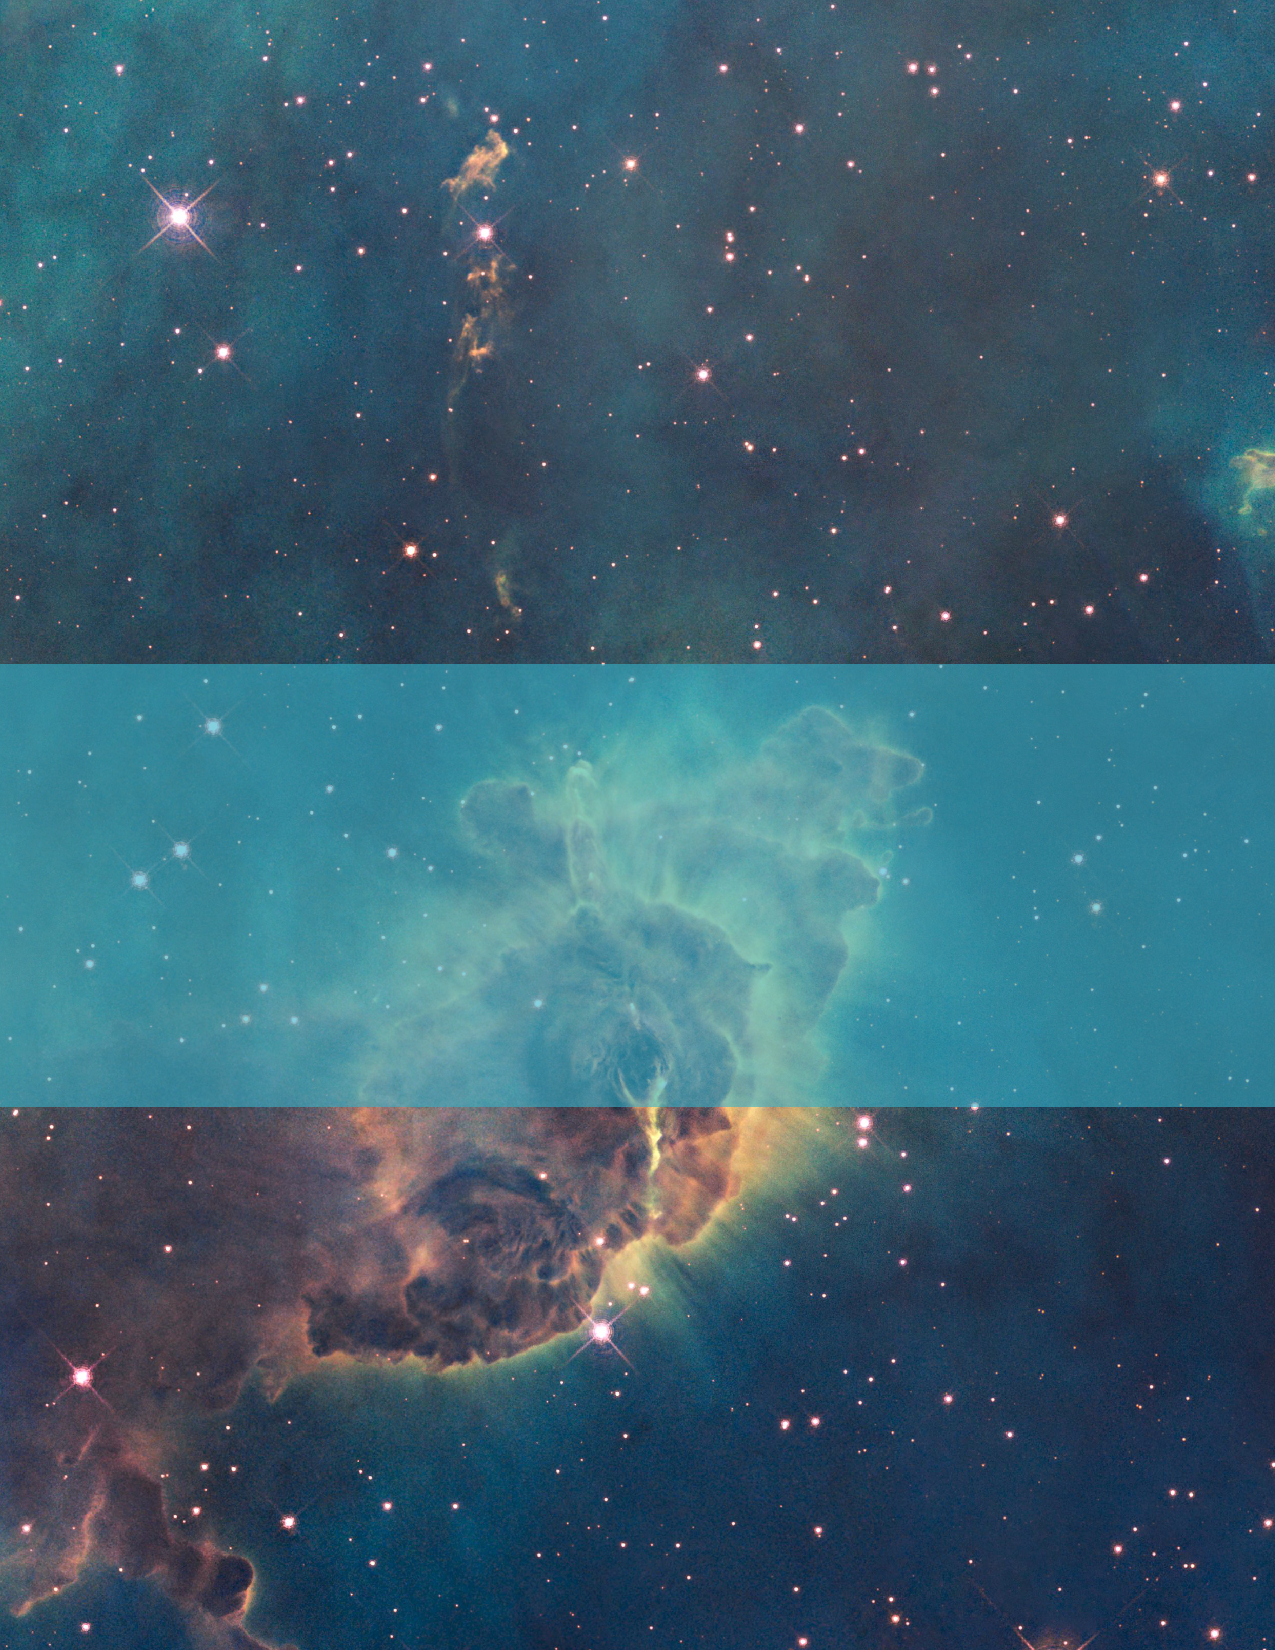
\includegraphics[scale=1.25]{esahubble}}} % Image background
\centering
\vspace*{5cm}
\par\normalfont\fontsize{35}{35}\sffamily\selectfont
\textbf{SymPy par la pratique(DRAFT(wip))}\\
{\LARGE Exemple et exercice avancée}\par % Book title
\vspace*{1cm}
{\Huge K.I.A Derouiche}\par % Author name
\endgroup

%----------------------------------------------------------------------------------------
%	COPYRIGHT PAGE
%----------------------------------------------------------------------------------------

\newpage
~\vfill
\thispagestyle{empty}

\noindent \textsc{github.com/kiaderouiche/misc}\\ % URL

%\noindent \textit{First release, August 2014} % Printing/edition date

%----------------------------------------------------------------------------------------
%	TABLE OF CONTENTS
%----------------------------------------------------------------------------------------

\chapterimage{head1.png} % Table of contents heading image

\pagestyle{empty} % No headers

\tableofcontents % Print the table of contents itself

%\cleardoublepage % Forces the first chapter to start on an odd page so it's on the right

\pagestyle{fancy} % Print headers again

%----------------------------------------------------------------------------------------
%	AVANT PROPOS
%----------------------------------------------------------------------------------------

\section{Avant-Propos}
Ce livre traite de SymPy, une bibliothèque de calcul symbolique entièrement écrite en Python un langage 
de programmation de haut niveau, orienté objet, totalement libre, conçu pour produire 
du code de qualité, portable et facile à intégrer. Ainsi la conception d'un programme scientifique  ou 
symbolique avec SymPy et Python est très rapide et offre au développeur une bonne productivité. En tant 
que bibliothèque pythonienne elle repose sur un langage dynamique, très souple d'utilisation et 
constitue un complément idéal à des langages compilés. Elle reste une bibliothèque complète et autosuffisant, pour des petits scripts fonctionnels de quelques lignes, comme pour des applicatifs complexes de plusieurs centaines de modules.

\subsection*{Pourquoi ce livre ?}
Il n'existe pas beaucoup d'ouvrages qui traitent du calcul symbolique en générale par  
rapport aux calculs numériques ou des ouvrages consacré aux bibliothèques symbolique écrite en Python 
est en particulier gravitent autour de SymPy mis à part un livre de 50 pages, quelques chapitres ou des 
lignes de codes cité à titre d'exemples. Citons le livre de référence de Svein Linge et Hans Petter 
Langtangen Programming for Computations – Python A Gentle Introduction to Numerical Simulations with 
Python, aux éditions Springer, ou encore une version du livre de 50 pages Instant SymPy Starter de Ronan 
Lamy, aux éditions Packt Publishing Limited, Le livre est Instant SymPy Starter de Ronan Lamy, c'est un 
guide de démarrage rapide, La documentation en ligne de SymPy est bonne, mais il serait plus facile de 
commencer avec ce livre. Alors, pourquoi ce livre ?

Si ce livre présente comme celui de Ronan Lamy les notions de la bibliothèque, celui-la ajoute des  
exemples originaux, des choix dans la présentation des classes, et une approche globale particulière et 
détaillé, il tente également d’ajouter à ce socle des éléments qui participent de la philosophie de la 
programmation en Python scientifique, aller plus loin dans le développement non scientifique, mettre en 
valeur L’Intérêt et l'importance, à savoir :
\begin{itemize}
 \item des conventions de codage ;
 \item combiné l'approche symbolique et numérique;
 \item des bonnes pratiques de programmation et des techniques d’optimisation ;
\end{itemize}

Même si chacun de ces sujets pourrait à lui seul donner matière à des ouvrages entiers, les réunir dans 
un seul et même livre contribue à fournir une vue complète de ce qu’un développeur d'application 
scientifique en particulier et Python averti et son chef de projet mettent en œuvre quotidiennement.

\subsection*{A qui s'adresse l'ouvrage?}
Cet ouvrage s’adresse bien sûr aux développeurs de tous horizons mais également aux
étudiants,chercheurs, enseignants et chefs de projets. Ils ne trouveront pas dans ce livre de bases de 
programmation; une pratique minimale préalable est indispensable de Python, quel que soit le langage 
utilisé. Il n’est pour autant pas nécessaire de maîtriser la programmation orientée objet et 
la connaissance d’un langage impératif est suffisante.
Les développeurs Python débutants – ou les développeurs avertis ne connaissant pas
encore cette bibliothèque – trouveront dans cet ouvrage des techniques et sujets avancées, les patterns 
efficaces et l’application de certains design patterns objet, topologie, théorie des catégories, machine
learning.
Les étudiants et enseignants trouveront un ouvrage ouvert sur l'apprentissage par l'exercice résolus et 
une interprétation d’exercices mathématiques  
les chercheurs trouveront un outil léger et efficace à travers des approches poussées liées aux 
questions récentes en connections avec les mathématiques pures et appliquées de physique théorique.
Les chefs de projets trouveront des éléments pratiques pour augmenter l’efficacité de
leurs équipes pluridisciplinaires, notamment la présentation des principaux modules à la fois issues de  la bibliothèque standard, graphique et numérique.

\chapterimage{head2.png} % Chapter heading image
\section{Premier pas vers SymPy}
Ce recueil d'exercices et de problèmes de programmation s'adresse aussi bien aux débutants qu'aux programmeurs confirmés. Il présente en effet plusieurs états d'esprit dont les deux principaux sont la programmation classique en Pascal pour les étudiants du premier cycle universitaire, et la programmation fonctionnelle en Lisp pour le second cycle.

Ce livre constitue un panorama (non exhaustif, mais suffisant) sur les langages de programmation, et offre une grande variété dans les sujets traités : graphiques, calcul matriciel, traitements de chaînes de caractères, graphes, intelligence artificielle...
\\
La première partie du livre sera consacré \`a la résolution par une approche symbolique au divers questions posées au étudiants et toute personnes qui aiment savoir et voir s'initier  pour des niveaux et des questions rencontrés, la deuxième partie du livre sera questions aux problèmes plus rencontrés pour des étudiants passionnée des questions entre mathématiques et technologies, chercheurs et développeurs d'applications scientifiques, la troisième partie plus consacré aux questions poussées

\subsection{Pourquoi programmer en symbolique }
Le symbolique est une grande importance d'un point de vue technique, car il permet
de limité les risques de bug dans l'exécution des programmes, dans le contexte de 
la vérification formelle si en prend le programme suivant:

\subsection{Calcul formel}

L'approche La simulation numérique est devenue essentielle dans de nombreux domaines tels que la mécanique des fluides et des solides, la météo, l'évolution du climat, la biologie ou les semi-conducteurs. Elle permet de comprendre, de prévoir, d'accéder là où les instruments de mesures s'arrêtent. 

Ce livre présente des méthodes performantes du calcul scientifique : matrices creuses, résolution efficace des grands systèmes linéaires, ainsi que de nombreuses applications à la résolution par éléments finis et différences finies. Alternant algorithmes et applications, les programmes sont directement présentés en langage C++. Ils sont sous forme concise et claire, et utilisent largement les notions de classe et de généricité du langage C++. 

Le contenu de ce livre a fait l'objet de cours de troisième année à l'école nationale supérieure d'informatique et de mathématiques appliquées de Grenoble (ENSIMAG) ainsi qu'au mystère de mathématiques appliquées de l'université Joseph Fourier. Des connaissances de base d'algèbre matricielle et de programmation sont recommandées. La maîtrise du contenu de cet ouvrage permet d'appréhender les principaux paradigmes de programmation du calcul scientifique. Il est alors possible d'appliquer ces paradigmes pour aborder des problèmes d'intérêt pratique, tels que la résolution des équations aux dérivées partielles, qui est abordée au cours de ce livre. La diversité des sujets abordés, l'efficacité des algorithmes présentés et leur écriture directe en langage C++ font de cet ouvrage un recueil fort utile dans la vie professionnelle d'un ingénieur. 

Le premier chapitre présente les bases fondamentales pour la suite : présentation du langage C++ à travers la conception d'une classe de quaternions et outils d'analyse asymptotique du temps de calcul des algorithmes. Le second chapitre aborde l'algorithme de transformée de Fourier rapide et développe deux applications à la discrétisation d'équations aux dérivées partielles par la méthode des différences finies. Le troisième chapitre est dédié aux matrices creuses et à l'algorithme du gradient conjugué. Ces notions sont appliquées à la méthode des éléments finis. En annexe sont groupés des exemples de génération de maillage et de visualisation graphique. 

S'il est cependant recommandé de maîtriser les notions du premier chapitre pour aborder le reste du livre, les chapitres deux et trois sont complètement indépendants et peuvent être abordés séparément. Ces chapitres sont complétés par des exercices qui en constituent des développements, ainsi que des notes bibliographiques retraçant l'historique des travaux et fournissant des références sur des logiciels et librairies récents implémentant ou étendant les algorithmes présentés. 

\subsection{Un peu de théorie}(source: Wikipédia)
Le calcul formel, ou parfois calcul symbolique, est le domaine des mathématiques et de informatique qui s'intéresse aux algorithmes opérant sur des objets de nature mathématique par le biais de représentations finies et exactes. Ainsi, un nombre entier est représenté de manière finie et exacte par la suite des chiffres de son écriture en base 2. Étant données les représentations de deux nombres entiers, le calcul formel se pose par exemple la question de calculer celle de leur produit.

Le calcul formel est en général considéré comme un domaine distinct du calcul scientifique, cette dernière appellation faisant référence au calcul numérique approché à l'aide de nombres en virgule flottante, là où le calcul formel met l'accent sur les calculs exacts sur des expressions pouvant contenir des variables ou des nombres en précision arbitraire (en). Comme exemples d'opérations de calcul formel, on peut citer le calcul de dérivées ou de primitives, la simplification d'expressions, la décomposition en facteurs irréductibles de polynômes, la mise sous formes normales de matrices, ou encore la résolution des systèmes polynomiaux.

Sur le plan théorique, on s'attache en calcul formel à donner des algorithmes avec la démonstration qu'ils terminent en temps fini et la démonstration que le résultat est bien la représentation d'un objet mathématique défini préalablement. Autant que possible, on essaie de plus d'estimer la complexité des algorithmes que l'on décrit, c'est-à-dire le nombre total d'opérations élémentaires qu'ils effectuent. Cela permet d'avoir une idée a priori du temps d'exécution d'un algorithme, de comparer l'efficacité théorique de différents algorithmes ou encore éclairer la nature même du problème.
\subsection{Logiciel de système de calcul formel}
Dans cette section en va exposer les systèmes de calcul formel, leur intérêt qui à vue un renouveau ces dernières années à cause de l'émergence de technique, technologie et nouvelle approche de programmation pour le domaine scientifique et industriel, hormis le fait que le logiciel de calcul formel en soient sont un outil pédagogique 
indispensable pour les scientifiques et les ingénieurs

\begin{definition}
Un logiciel de système formel est un outil qui facilite le calcul symbolique. La partie principale de ce système est la manipulation des expressions mathématiques sous leur forme symbolique.
\end{definition}

\begin{example}
soit $G=\{x\in\mathbb{R}^2:|x|<3\}$ et noté par: $x^0=(1,1)$; en considère la fonction:
\begin{equation}
f(x)=\left\{\begin{aligned} & \mathrm{e}^{|x|} & & \text{si $|x-x^0|\leq 1/2$}\\
& 0 & & \text{si $|x-x^0|> 1/2$}\end{aligned}\right.
\end{equation}
The function $f$ has bounded support, we can take $A=\{x\in\mathbb{R}^2:|x-x^0|\leq 1/2+\epsilon\}$ for all $\epsilon\in\intoo{0}{5/2-\sqrt{2}}$.
\end{example}

cet exemple se traduit en forme symbolique avec la bibliothèque SymPy:

\subsection{Quelques logiciels de calcul formel}

qui exprime ce qui nous permet notre choix pour un CAS qui possède des caractéristiques techniques et sur le plan du coût très important quand peut résumer dans les points suivants:
\begin{enumerate}
	\item Leger et 
	\item S’appuie sur le langage de programmation Python
	\item Portabilité dans toute transparence
\end{enumerate}

L'un des systèmes qui peut nous permettre d'écrire cette exemple avec un ordinateurs avec SymPy qui semble mieu intégré

\subsection{Bibliothèque SymPy}

Dans un cas plus simple l'exemple 1.1 se formule beaucoup plus dans un outil comme SymPy est une bibliothèque de calcul formel elle est aussi un environnement pour 
l’apprentissage de l’algèbre, l’analyse, géométrie, combinatoire, cryptographie, mécanique 
classique et quantique pour le lycée et l’université mais aussi un environnement de 
développement et de recherche. SymPy  écrit entièrement en Python un langage de 
programmation facile à apprendre et adapté à l’apprentissage,  elle fourni aux étudiant 
\textit{SymPyGamma} une application web   notamment des primitives générales de traitement des expressions algébriques (développement, factorisation, …), des aides à l’organisation des objets mathématiques intervenant dans la résolution d’un problème ainsi qu’une assistance à la preuve. Il permet au professeur de préparer et de suivre le travail de l’élève. Différentes maquettes ont été développées et testées auprès d’élèves. Dans la plus récente, nous nous sommes attachés à explorer une nouvelle forme d’activité algébrique. Alors que le calcul en papier crayon et les logiciels standards considèrent
 les expressions de façon isolée, l’environnement que nous développons organise en réseau les différentes expressions intervenant dans la résolution d’un problème. L’ordinateur peut facilement mettre à jour ce réseau quand l’utilisateur modifie certains de ses éléments. Il devient ainsi possible, pour aborder un problème générique, d’explorer facilement des cas particuliers et de conduire une généralisation. Les relations entre expressions algébriques sont mieux mises en évidence du fait de leur invariance dans les modifications du réseau. De façon très concise, Casyopée peut être défini
\subsubsection{SymPyGamma}
Est une interface onWeb marche avec un navigateur contient plusieurs catégorie liée de calcul, dynamique. L’Intérêt de cette outil qu'il est facilement partageable adapté pour l’enseignement et surtout l'auto-apprentissage 
\subsubsection{Besoin de rester dans le symbolique}
Le symbolique est une grande importance d'un point de vue technique, car il permet
de limité les risques de bug dans l'exécution des programmes, dans le contexte de 
la vérification formelle si en prend le programme suivant:

\subsubsection{Passage du symbolique au numérique}
Généralement, le symbolique parmi c'est  
\subsection{Faire des dessins}



%----------------------------------------------------------------------------------------
%	CHAPTER 1
%----------------------------------------------------------------------------------------
\part{Premier pas vers SymPy}
\chapter{Premier pas vers SymPy}

Ce chapitre d’introduction présente la tournure d'esprit de la bibliothèque mathématique SymPy. Les 
autres chapitres de cette partie développent les notions de base de SymPy: effectuer des calculs 
numériques ou symboliques en analyse, opérer sur des vecteurs et des matrices, écrire des programmes, 
manipuler des listes de données, construire des graphiques, etc. Les parties suivantes de cet ouvrage 
approfondissent quelques branches des mathématiques dans lesquelles l'informatique fait preuve d'ne 
grande efficacité.

\section{La bibliothèque SymPy}

\subsection{Le cas de la bibliothèque SymPy}

Dans un cas plus simple l'exemple 1.1 se formule beaucoup plus dans un outil comme SymPy est une bibliothèque de calcul formel elle est aussi un environnement pour 
l’apprentissage de l'algèbre, l’analyse, géométrie, combinatoire, cryptographie, mécanique 
classique et quantique pour le lycée et l’université mais aussi un environnement de 
développement et de recherche. SymPy  écrit entièrement en Python un langage de 
programmation facile à apprendre et adapté à l’apprentissage,  elle fourni aux étudiant 
\textit{SymPyGamma} une application web   notamment des primitives générales de traitement des 
expressions algébriques (développement, factorisation, …), des aides à l’organisation des objets 
mathématiques intervenant dans la résolution d’un problème ainsi qu’une assistance à la preuve. Il 
permet au professeur de préparer et de suivre le travail de l’élève. Différentes maquettes ont été 
développées et testées auprès d’élèves. Dans la plus récente, nous nous sommes attachés à explorer une 
nouvelle forme d’activité algébrique. Alors que le calcul en papier crayon et les logiciels standards 
considèrent  les expressions de façon isolée, l’environnement que nous développons organise en réseau 
les différentes expressions intervenant dans la résolution d’un problème. L’ordinateur peut facilement 
mettre à jour ce réseau quand l’utilisateur modifie certains de ses éléments. Il devient ainsi possible, 
pour aborder un problème générique, d’explorer facilement des cas particuliers et de conduire une 
généralisation. Les relations entre expressions algébriques sont mieux mises en évidence du fait de leur 
invariance dans les modifications du réseau. De façon très concise, Casyopée peut être défini
\subsection{Travaillez avec SymPy}
\subsection{Installation de SymPy}

\subsection{isympy}
  \begin{python}
IPython console for SymPy 1.3 (Python 3.6.7-64-bit) (ground types: python)
These commands were executed:
>>> from __future__ import division
>>> from sympy import *
>>> x, y, z, t = symbols('x y z t')
>>> k, m, n = symbols('k m n', integer=True)
>>> f, g, h = symbols('f g h', cls=Function)
>>> init_printing()

Documentation can be found at http://docs.sympy.org/1.3/

  \end{python}
\subsection{SymPyGamma}
Est une interface onWeb marche avec un navigateur contient plusieurs catégorie liée de calcul, dynamique. L’Intérêt de cette outil qu'il est facilement partageable adapté pour l’enseignement et surtout l'auto-apprentissage

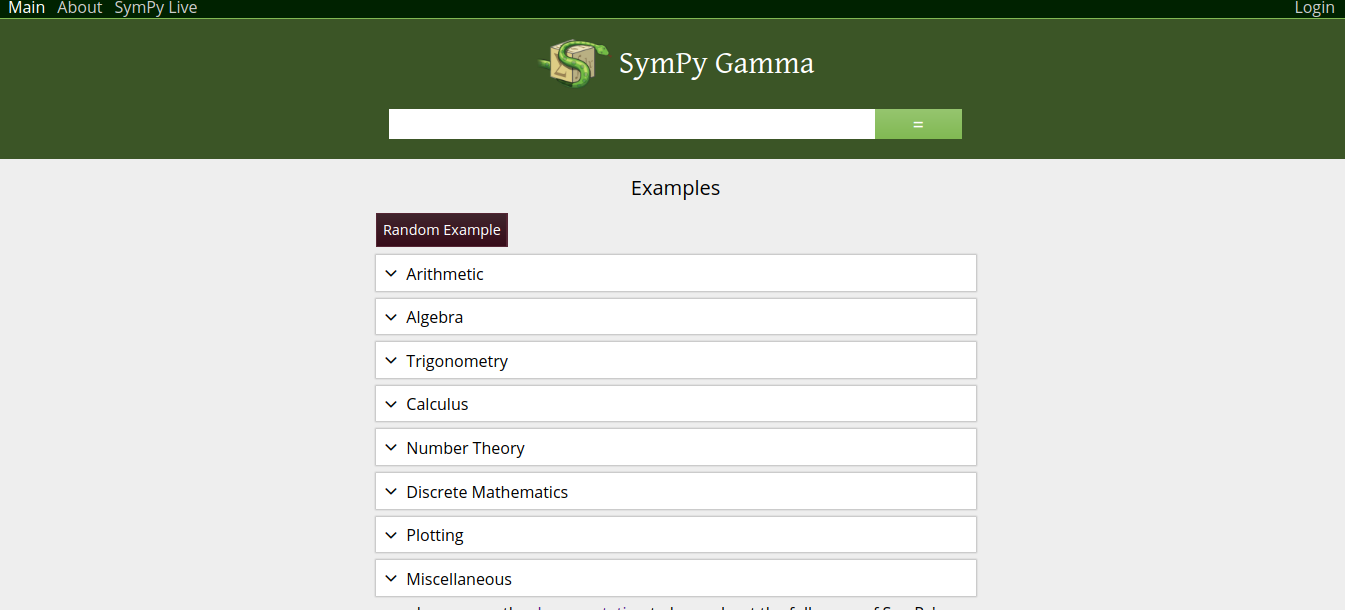
\includegraphics[scale=0.3]{../Pictures/sympyGammaMain.png} 

\subsection{SymPyLive}
SymPy Live est SymPy qui s'exécute sur Google App Engine. Ceci est juste un shell Python standard, avec les commandes suivantes exécutées par défaut
\section{SymPy comme calculatrice}
Contrairement à Sage[], Maple, Octave et les autres logiciel de calcul formel, SymPy, effectue des calculs directe numériques de deux manière différents en passant par la méthode, 
\subsection{Premier calculs}
Dans la suite du livre, nous présentons les calculs sous la forme suivante, qui
imite l’allure d’une session de SymPyLive à travers la ligne de commande isympy:
\begin{python}
In [1]: from sympy import *
In [2]: 1+1                                                                     
Out[2]: 2
\end{python}
\subsubsection{Variables Python}
Lorsque l’on veut conserver le résultat d’un calcul, on peut l’affecter à une
variable :

\subsubsection{Variables Symboliques}
Les objets mathématiques manipulés par SymPy sont symboliques ils sont représentés exactement loin de 
toute approximation numérique, SymPy permet une manipulation avec des expressions contenant
des variables, comme $x^{2} + zy^{3} + z^{2}$ ou encore $sin(x) - exp(x)$. Les variables symboliques
du mathématicien $x$, $y$, $z$ apparaissant dans ces expressions diffèrent, avec SymPy,
des variables du développeur $sin(2) = 0.9092974268256817$ que nous manipulons sous Python 
section précédente. SymPy diffère notablement, sur ce point, d’autres systèmes de calcul
formel comme Maple ou Maxima, Sage c'est inspiré de SymPy sur ce point.
\\

La documentation officiel présente la différence entre valeur numérique gérer par la bibliothèque
standard Python math à travers l'exemple de la racine carré $\sqrt{8}$ sans évaluation,
posons $x=8$

\begin{python}
In [1]: import math                                                             
In [2]: math.sqrt(x)                                                            
Out[2]: 2.8284271247461903
\end{python}
Les variables symboliques doivent \^etre explicitement déclarées avant d'\^etre employées

Dans cet exemple, la commande SR.var(’z’) « construit » et renvoie une variable symbolique dont le nom est z. Cette variable symbolique est un objet Sage comme un autre : elle n’est pas traitée différemment d’expressions plus complexes comme $sin(x) + 1$. Ensuite, cette variable symbolique est affectée à la variable « du programmeur » z, ce qui permet de s’en servir comme de n’importe quelle expression pour construire des expressions plus complexes.


\begin{python}
In [1]: from sympy import *
In [2]: x = symbols('x')                                                                     
In [3]: type(x)
Out[3]: sympy.core.symbol.Symbol
\end{python}

\begin{python}
In [4]: x+3                                                                     
Out[4]: x + 3
\end{python}

\subsection{Structure de données dans SymPy}
Le moteur symbolique de SymPy tire parti de l'orientation des objets (notamment l'héritage) pour créer une base de code facilement extensible. Toutes les classes dérivent des fonctionnalités, telles que la possibilité de se comparer à d'autres objets, à partir de méthodes de la super-classe Basic. Les objets pouvant faire l'objet d'opérations algébriques acquièrent cette capacité grâce à un ensemble de méthodes d'une classe appelée Expr. Ces objets Expr peuvent être conservés dans des objets conteneur (qui contiennent également la sous-classe Expr) Mul, Add et Pow; les objets conteneur sont instanciés à l'aide de l'opérateur Python, tel que la fonction de surcharge, qui permet au constructeur de la classe conteneur d'être appelé chaque fois que l'opérateur binaire approprié est utilisé (* pour Mul, + pour Ajouter et $**$ pour Pow).
De cette manière, des objets supplémentaires peuvent être ajoutés en créant simplement une sous-classe qui hérite des fonctionnalités de la classe Expr. Ces sous-classes bénéficient gratuitement de certaines fonctionnalités, telles que la possibilité de comparer, de multiplier, d’ajouter, etc. Voici comment SymPy crée un environnement modifiable, maintenable, et donc facile à étendre. Grâce à la possibilité d'hériter des propriétés de classes supérieures, la quantité de code nécessaire pour développer, par exemple, un système modélisant la mécanique quantique et la notation Dirac décroissant de manière significative.

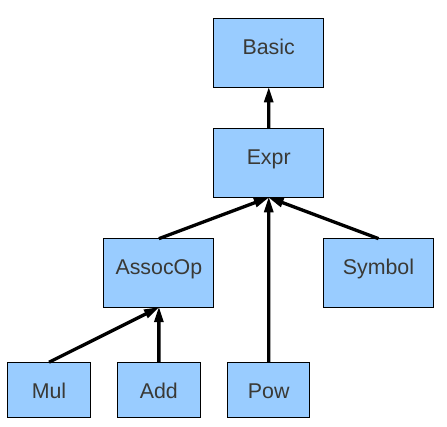
\includegraphics[scale=0.5]{../Pictures/sympyarch.png} 
\subsection{Variable et affection}\index{Variable et affection}

\begin{exercise}
Affectez les variables temps $t$ et distance $d$ par les valeurs 6.892 et 19.7. Calculez et affichez la valeur de la vitesse. Améliorez l'affichage en imposant un chiffre après le point décimal.
\end{exercise}

\begin{solution}
Pour, affectez des variables est les rendre symbolique comme c'est décrit dans le mémo ou il 
sera expliquer temps $t$ et distance $d$ par les valeurs 6.892 et 19.7. Calculez et affichez la 
valeur de la vitesse. Améliorez l'affichage en imposant un chiffre après le point décimal.
\end{solution}

\subsection{Substitution}
Une des choses les plus courantes que vous pourriez vouloir faire avec une expression mathématique est la substitution. La substitution remplace toutes les occurrences de quelque chose dans une expression par quelque chose d'autre. SymPy utilisant la méthode \textbf{subs}. Sym

\subsection{Contrôle du flux d’instructions}\index{Theorems!Single Line}
This is a theorem consisting of just one line.

\begin{exercise}
A set $\mathcal{D}(G)$ in dense in $L^2(G)$, $|\cdot|_0$. 
\end{exercise}
\begin{solution}
\end{solution}
%------------------------------------------------

\chapter{Analyse et Algèbre}\index{Analyse et Algèbre}
Ce chapitre présente à travers des exemples simples les fonctions de base utiles en analyse et en algèbre. Les 
lycéens et étudiants trouveront matière à  remplacer le crayon et le papier par le clavier et l'écran tout en 
relevant le même défi intellectuel de compréhension des mathématiques.Cet exposé des principales commandes de calcul 
avec Sage se veut accessible aux élèves de lycée.

\section{Expressions symboliques et simplification}\index{Expressions symboliques et simplification}
 \subsection{Expressions symboliques}
La bibliothèque SymPy permet d'effectuer toutes sortes de calculs d'analyse à partir d'expressions
symboliques combinant des nombres, des variables symboliques, les quatre opérations, et des fonctions usuelles comme 
sqrt, exp, log, sin, cos, etc. Une expression symbolique peut être représentée par un arbre comme ceux de la. Il est 
important de comprendre qu'une expression symbolique est une formule et non pas une valeur ou une fonction 
mathématique. Ainsi, SymPy ne reconnaît pas que les deux expressions suivantes sont égales
\subsection{Transformation d'expressions}\index{Transformation d'expressions}
\subsection{Fonctions mathématiques usuelles}\index{Fonctions mathématiques usuelles}
La plupart des fonctions mathématiques se retrouvent dans SymPy, en particulier les
fonctions trigonométriques, le logarithme et l'exponentiel : elles sont rassemblées
dans le tableau

\section{Équations}
Ceci est la documentation officielle du module solveset dans les solveurs. Il contient les questions fréquemment posées sur notre nouveau module pour résoudre des équations.
 \subsection{Résolution explicite}\index{Résolution explicite}
 \subsection{Équations sans solution explicite}\index{Équations sans solution explicite}
\section{In\'equations}\index{In\'equations}
\section{Analyse}\index{Analyse}
Dans cette section, nous présentons succinctement les fonctions couramment utiles en analyse réelle. Pour une 
utilisation avancée ou des compléments, on renvoie aux chapitres suivants notamment ceux qui traitent de 
l'intégration numérique (ch. 14), de la résolution des équations non linéaires (ch. 12), et des
équations différentielles (ch. 10)
 \subsection{Les Fonctions}\index{Fonctions}
Il sert également de constructeur pour les classes de fonctions non définies.

\begin{python}
from sympy import Function, Symbol
\end{python}

\begin{exercise}
Écrire une fonction cube qui retourne le cube de son argument
\end{exercise}

\begin{exercise}
Écrire une fonction $volumeSphere$ qui calcule le volume d’une sphère de rayon $r$ fourni
en argument et qui utilise la fonction cube .
Tester la fonction $volumeSphere$ par un appel dans le programme principal.
\end{exercise}

\begin{exercise}
Écrire une fonction maFonction qui retourne $f(x) = 2x^{3} + x - 5$
\end{exercise}

\begin{exercise}
Écrire une fonction tabuler avec quatre paramètres : $fonction$ , $borneInf$ , $borneSup$
et $nbPas$ . Cette procédure affiche les valeurs de $fonction$ , de $borneInf$ à $borneSup$ ,
tous les nbPas . Elle doit respecter $borneInf < borneSup$.
Tester cette fonction par un appel dans le programme principal après avoir saisi les
deux bornes dans une floatbox et le nombre de pas dans une integerbox (utilisez le
module easyguiB ).
\end{exercise}

\begin{exercise}
Écrire une fonction $volMasse$ Ellipsoide qui retourne le volume et la masse d'un ellipsoïde grâce à un tuple. Les paramètres sont les trois demi-axes et la masse volumique. On donnera à ces quatre paramètres des valeurs par défaut. \\
On donne: $v = \frac{3}{4} \pi abc$ \\
Tester cette fonction par des appels avec différents nombres d'arguments.
\end{exercise}

\begin{exercise}
Une fonction $f (x)$ est lin\'eaire et a une valeur de $29$ \`a $x = -2$ et $39$ à $x = 3$. Trouver sa valeur à $x = 5$.
\end{exercise}

\begin{exercise}
Pour l'ensemble $N$ de nombres naturels et une opération binaire $f: N x N \longrightarrow N$, on appelle un élément $z$ $\epsilon$ $N$ une identité pour $f$, si $f (a, z) = a = f (z, a)$, pour tout a $\epsilon$ $N$. Lesquelles des opérations binaires suivantes ont une identité?:
\begin{enumerate}
  \item $f (x, y) = x + y - 3$
  \item $f (x, y) = max(x, y)$
  \item $f (x, y) = x^{y}$
\end{enumerate}
\end{exercise}
\begin{solution}
le deuxième et le troisième 
\end{solution}
 \subsection{Sommes}
 \subsection{Limites}
 \subsection{Suites}
 \subsection{Développements limités}
 \subsection{Séries}
  On peut utiliser les commandes précédentes pour effectuer des calculs sur les séries. Donnons quelques exemples.
 \subsection{Dérivation}
 La fonction derivative (qui a pour alias diff) permet de dériver une expression symbolique ou une fonction symbolique
 \subsection{Dérivées partielles}
 La commande diff permet également de calculer des dérivées n-ièmes ou des dérivées partielles.
 \subsection{Intégration}
 \section{Calcul matriciel}
  Dans cette section, on décrit les fonctions de base utiles en algèbre linéaire :opérations sur les vecteurs, puis sur les matrices. Pour plus de détails, on renvoie au chapitre 8 pour le calcul matriciel symbolique et au chapitre 13 pour le calcul matriciel numérique.
  \subsection{Résolution de systèmes linéaires}\index{Résolution de systèmes linéaires}
  \subsection{Calcul vectoriel}\index{Calcul vectoriel}
  Les fonctions de base utiles pour la manipulation des vecteurs sont résumées dans le tableau 2.5. On peut se servir de ces fonctions pour traiter l'exercice suivant.
  \subsection{Calcul matriciel} \index{Calcul matriciel}
  \subsection{Réduction d'une matrice carrée}\index{Réduction d'une matrice carrée}
 \chapter{Graphiques}
La visualisation de fonctions d'une ou deux variables, d'une série de données, facilite la perception de phénomènes mathématiques ou physiques et permet de conjecturer des résultat Équations sans solution explicitement efficacement. Dans ce chapitre, on illustre sur des exemples les capacités graphiques de SymPy.
 \section{Courbes en 2D}\index{Courbes en 2D}
 Une courbe plane peut être définie de plusieurs façons : comme graphe d'une fonction d'une variable, par un système d'équations paramétriques, par une équation en coordonnées polaires, ou par une équation implicite. Nous présentons
ces quatre cas, puis donnons quelques exemples de tracés de données.
 \subsection{Représentation graphique de fonctions}\index{Représentation graphique de fonctions}
 \subsection{Courbe paramétrée}\index{Courbe paramétrée}
 Les tracés de courbes paramétrées $(x = f(t), y=g(t))$ sont réalisés par la commande Curve\footnote{du module sympy.geometry(quand on le verra dans le chapitre)}$((f(t), g(t)), (t, a, b))$ ou $\left[a, b\right]$ est l'intervalle parcouru par le paramètre.
 \\
 Représentons par exemple la courbe paramétrée d'équations :
  
 \subsection{Courbe en coordonnées polaires}\index{Courbe en coordonnées gpolaires}
 \subsection{Courbe définie par une équation implicite}\index{Courbe définie par une équation implicite}
 Pour représenter une courbe donnée par une équation implicite, on utilise la fonction \textbf{plot\_implicit}
 $(f(x, y), (x, a, b), (y, c, d))$
 \subsection{Tracé de données}\index{Tracé de données}
 \subsection{Tracé de solution d'équation différentielle}\index{Tracé de solution d'équation différentielle}
 
 \subsection{Développée d'une courbe}\index{Développée d'une courbe}
 \section{Courbes en 3D}   

%----------------------------------------------------------------------------------------
%	CHAPTER 2
%----------------------------------------------------------------------------------------
\subsection{Nombres parfaits et nombres chanceux}
En mathématique un nombre chanceux est un entier naturel dans un ensemble qui est généré par un « crible » similaire au crible d'Ératosthène qui génère les nombres premiers
\begin{exercise}
$\sqrt{12}$
\end{exercise}
%------------------------------------------------

\section{Examples}\index{Examples}

This is an example of examples.

\subsection{Equation and Text}\index{Examples!Equation and Text}

\begin{example}
Let $G=\{x\in\mathbb{R}^2:|x|<3\}$ and denoted by: $x^0=(1,1)$; consider the function:
\begin{equation}
f(x)=\left\{\begin{aligned} & \mathrm{e}^{|x|} & & \text{si $|x-x^0|\leq 1/2$}\\
& 0 & & \text{si $|x-x^0|> 1/2$}\end{aligned}\right.
\end{equation}
The function $f$ has bounded support, we can take $A=\{x\in\mathbb{R}^2:|x-x^0|\leq 1/2+\epsilon\}$ for all $\epsilon\in\intoo{0}{5/2-\sqrt{2}}$.
\end{example}
%------------------------------------------------------------------------------
%	CHAPTER 3
%----------------------------------------------------------------------------------------

\section{Programmation Orientée Objet}\index{Notations}
\begin{notation}
Given an open subset $G$ of $\mathbb{R}^n$, the set of functions $\varphi$ are:
\begin{enumerate}
\item Bounded support $G$;
\item Infinitely differentiable;
\end{enumerate}
a vector space is denoted by $\mathcal{D}(G)$. 
\end{notation}

 \subsection{POO}
\begin{exercise}
 Définir une classe Vecteur2D avec un constructeur fournissant les coordonnées par
défaut d’un vecteur du plan (par exemple : $x = 0$ et $y = 0$ ).
Dans le programme principal, instanciez un Vecteur2D sans paramètre, un Vecteur2D
avec ses deux paramètres, et affichez-les.
\end{exercise}
\begin{solution}
 en utilise le module sympy.geometry ce module fait appel à tout les outils et theories qui
 peuvents entre utiliser dans le cade de la géométrie dans le Plan.
 \begin{python}
 from sympy.geometry
  \end{python}
\end{solution}

\begin{exercise}
Enrichissez la classe Vecteur2D précédente en lui ajoutant une méthode d’affichage
et une méthode de surcharge d’addition de deux vecteurs du plan.
Dans le programme principal, instanciez deux Vecteur2D , affichez-les et affichez leur
somme.
\end{exercise}
\begin{solution}
\end{solution}

%------------------------------------------------
\subsection{Notions de COO et d’encapsulation}
%------------------------------------------------

%%
%\includeonly{geometry/euclid}


\section{Remarks}\index{Remarks}

This is an example of a remark.

\begin{remark}
The concepts presented here are now in conventional employment in mathematics. Vector spaces are taken over the field $\mathbb{K}=\mathbb{R}$, however, established properties are easily extended to $\mathbb{K}=\mathbb{C}$.
\end{remark}

%------------------------------------------------

\section{Corollaries}\index{Corollaries}

This is an example of a corollary.

\begin{corollary}[Corollary name]
The concepts presented here are now in conventional employment in mathematics. Vector spaces are taken over the field $\mathbb{K}=\mathbb{R}$, however, established properties are easily extended to $\mathbb{K}=\mathbb{C}$.
\end{corollary}

%------------------------------------------------

\section{Propositions}\index{Propositions}

This is an example of propositions.

\subsection{Several equations}\index{Propositions!Several Equations}

\begin{proposition}[Proposition name]
It has the properties:
\begin{align}
& \big| ||\mathbf{x}|| - ||\mathbf{y}|| \big|\leq || \mathbf{x}- \mathbf{y}||\\
&  ||\sum_{i=1}^n\mathbf{x}_i||\leq \sum_{i=1}^n||\mathbf{x}_i||\quad\text{where $n$ is a finite integer}
\end{align}
\end{proposition}

\subsection{Single Line}\index{Propositions!Single Line}

\begin{proposition} 
Let $f,g\in L^2(G)$; if $\forall \varphi\in\mathcal{D}(G)$, $(f,\varphi)_0=(g,\varphi)_0$ then $f = g$. 
\end{proposition}

\subsection{Paragraph of Text}\index{Examples!Paragraph of Text}

\begin{example}[Example name]
\lipsum[2]
\end{example}

%------------------------------------------------

\section{Exercises}\index{Exercises}

This is an example of an exercise.

\begin{exercise}
This is a good place to ask a question to test learning progress or further cement ideas into students' minds.
\end{exercise}

%------------------------------------------------

\section{Problems}\index{Problems}

\begin{problem}
What is the average airspeed velocity of an unladen swallow?
\end{problem}

%------------------------------------------------

\section{Vocabulary}\index{Vocabulary}

Define a word to improve a students' vocabulary.

\begin{vocabulary}[Word]
Definition of word.
\end{vocabulary}


%---------------------------------------------------------------------------------------
%	CHAPTER 3
%----------------------------------------------------------------------------------------
\chapter{Problème non linéaire}
Les sujets de ce chapitre sont du néanmoins axées sur des questions ou l'approche mathématique et 
physique et demandé 

\section{Chaos}\index{Mouvement d'un pendule}
Prenons une pause dans l'apprentissage de nouvelles techniques et algorithmes informatiques
pour un peu, et passer du temps en utilisant ce que nous avons appris jusqu'à présent pour enquêter sur quelque chose d'intéressant. Nous allons commencer avec quelque chose de familier: le simple pendule.
\subsection{Pendule simple}
Le pendule simple figure
\subsection{Pendule à deux bras}
\subsection{Mouvements d’un robot}
Qu'est ce qu'il faut savoir quand en veut modélisé le comportement d'un robot?. Et bien la réponse est tout simplement des mathématiques

\section{M\'ecanique et information quantique}
\section{Le modèle $\phi^{4}$}
 \subsection{LES DIAGRAMMES DE FEYNMAN}
 
\section{Solution non linéaire d'équation algébrique}\index{Solving Nonlinear Algebraic Equations}

Qu'est ce que non-linéaire et qu'est ce que une \'equation alg\'ebrique

Une \'equation alg\'ebrique est un polyn\^ome de la forme $P(x)$

\begin{equation}
\exp(-x)\sin(x) = \cos(x)
\end{equation}

%-------------------------------------------------------------------------------------------------
% CHAPTER 4
%-------------------------------------------------------------------------------------------------
\chapter{Mathématique pures}
\section{La théorie de catégorie}
L'interet de la théorie de catégorie dans les mathématiques modernes et l'informatique théorique et sui dépasse de loin, cette derniére pour \^etre
\section{Transport optimal}
C'est quoi le \textit{ transport optimal}?, exemple simple..., le domaine du transport optimal
est très 
%-------------------------------------------------

\section{Figure}\index{Figure}

\begin{table}[h]
\centering
\begin{tabular}{l l l}
\toprule
\textbf{Treatments} & \textbf{Response 1} & \textbf{Response 2}\\
\midrule
Treatment 1 & 0.0003262 & 0.562 \\
Treatment 2 & 0.0015681 & 0.910 \\
Treatment 3 & 0.0009271 & 0.296 \\
\bottomrule
\end{tabular}
\caption{Table caption}
\end{table}

%
%\begin{figure}[h]
%\centering\includegraphics[scale=0.5]
%\caption{Figure caption}
%\end{figure}

%----------------------------------------------------------------------------------------
%	Technique Avancée
%----------------------------------------------------------------------------------------

\chapter{Annexe}

\section{Programmation Orientée Objet}\index{Notations}
\section{D\'ecorateurs}
Les d\'ecorateurs un m\'ecanisme incontournable pour \'ecrire de tr\'es bon code et purement 
lisible et portable
\subsection{Optimisation du code}
Sans aucun doute l'usage de la programmation symbolique avec ce que en a vue plus haut, ralentisse grandement l'exécution du programme, donc en gagne sur le coté sureté, élégance
et maintenance du code et d'autre part en perd complètement la vitesse; penser à des centaine de ligne de code si vous voulez programmé un robot, voiture ou des objets connectés qui implémente des algorithmes mathématiques et qui de demande beaucoup de ressource est un temps de retour très élevées 

\subsection{Cython}
Cython (http://www.cython.org/ ) est un métalangage qui permet de combiner du code
Python et des types de donn\'ees C, pour concevoir des extensions compilables pour
Python.
Dans un module Cython, il est possible de définir des variables C directement dans
le code Python et de définir des fonctions C qui prennent en paramètre des
variables C ou des objets Python.
Cython contr\^ole ensuite de manière transparente la génération de l’extension C, en
transformant le module en code C par le biais des API C de Python.
Toutes les fonctions Python du module sont alors automatiquement publiées.
Le gain de temps dans la conception introduit par Cython est considérable : toute la
mécanique habituellement mise en œuvre pour créer un module d’extension est
entièrement gérée par Cython.
Ainsi, la fonction max() du module calculs.c pr\'ec\'edemment présent\'ee devient :

Les fichiers Cython ont par convention l’extension pyx, en référence à l’ancien nom.

setup.py pour calculs.pyx

\begin{python}
from distutils.core import setup
from distutils.extension import Extension
from Cython.Distutils import build_ext

extension = Extension("calculs", ["calculs.pyx"])

setup(name="calculs", ext_modules=[extension],cmdclass={'build_ext': build_ext})

\end{python}

\subsection{Theano}
Theano est une biblioth\'eque pour l'acc\e'ration du code lent en Python, tr\'es importante et intéressante
elle offre une syntaxe très particulière.
\section{Interface graphique}
Quelle bibliothèque choisir: sous Python en \`a le choix entre diff\'erente, Tkinter, Gtk, 
Qt, wx et ftk, et il existe encore d'autre bibliothèques qui sont con\c{c}u pour le calcul 
et application scientifique \'editer par Thought[...] dans cette section nous allons. Une 
autre approche serait d'utiliser les ipywdigets avec Jupyter ou JupyterLab notebook, les 
ipywidgets sont trés intéressante approches pour des graphiques interactives rapide d'usages
et bénéfiques sur le plan de présentation par exemple quand en veut exporté ou les partagés 

\section{Bibliographie}
\section{Index}

\end{document}
